\section{Platforms and Models}
\subsection{JuPedSim and Social Force Model}
JuPedSim \cite{chraibiJuPedSim2025} is an open-source software framework for pedestrian dynamics and personnel evacuation simulation, aiming to study the movement and evacuation behaviors of people in the built environment through computer simulation. This tool takes "self-driven multi-agent system" as its core concept, modeling each pedestrian as an independent agent. The agents follow a set of rules in a given scene to determine their own movement path, speed and interaction behavior, thereby presenting phenomena such as flow, congestion, queuing and path selection at the group level at the macro level. 

JuPedSim is assembled with pedestrian dynamics models such as the classic Social Force Model. The model defines three forces that influence pedestrian movement: the driving force, the repulsive force between pedestrians, and the repulsive force from obstacles. The driving force represents the agent's desire to reach a target position at a certain speed, while the repulsive force is caused by the interaction between the individuals and causes them to avoid each other in order to avoid collisions.The obstacle force acts in a similar way to the repulsive force to avoid collisions with obstacles.

The fundamental principle can be expressed by the following equation:
\begin{equation}
    m_i\underbrace{\frac{d\boldsymbol{v}_i}{dt}}_{\text{Acceleration}} = \underbrace{m_i \frac{\boldsymbol{v}_i^0(t)\boldsymbol{e}_i^0(t) - \boldsymbol{v}_i(t)}{\tau_i}}_{\text{Driving Force}} + \underbrace{\sum_{j(\neq i)} f_{ij} + \sum_W f_{iW}}_{\text{Interaction Forces}}
\end{equation}

Where \(m_i\) is the mass of pedestrian \(i\), \(\boldsymbol{v}_i(t)\) is the current velocity, \(\boldsymbol{v}_i^0(t)\) is the desired speed, \(\boldsymbol{e}_i^0(t)\) is the desired direction, and \(\tau_i\) is the relaxation time. The terms \(f_{ij}\) and \(f_{iW}\) represent the repulsive forces from other pedestrians and obstacles, respectively.

Specifically, the repulsive force between pedestrians \(f_{ij}\) can be expressed as:
\begin{equation}
    f_{ij}^{repulsive} = \underbrace{A_i \exp\left(\frac{r_{ij} - d_{ij}}{B_i}\right) \mathbf{n}_{ij} + k g(r_{ij} - d_{ij}) \mathbf{n}_{ij}}_{\text{Pushing}} + \underbrace{\kappa g(r_{ij} - d_{ij}) \Delta v_{ji}^t \mathbf{t}_{ij}}_{\text{Friction}}
\end{equation}

Where \(A_i\) and \(B_i\) are constants representing the strength and range of the repulsive force, \(r_{ij}\) is the sum of the radii of pedestrians \(i\) and \(j\), \(d_{ij}\) is the distance between them, \(\mathbf{n}_{ij}\) is the unit vector pointing from pedestrian \(j\) to \(i\), \(\mathbf{t}_{ij}\) is the tangential unit vector, \(k\) and \(\kappa\) are constants related to body compression and friction, and \(g(x)\) is a function that equals \(x\) if \(x > 0\) and 0 otherwise.

The obstacle force from  \(f_{iW}\) is similarly defined as:
\begin{equation}
    f_{iW}^{obstacle} = \underbrace{A_i \exp\left(\frac{r_i - d_{iW}}{B_i}\right) \mathbf{n}_{iW} + k g(r_i - d_{iW}) \mathbf{n}_{iW}}_{\text{Pushing}} + \underbrace{\kappa g(r_i - d_{iW}) (\mathbf{v}_i \cdot \mathbf{t}_{iW}) \mathbf{t}_{iW}}_{\text{Friction}}
\end{equation}

Where \(r_i\) is the radius of pedestrian \(i\), \(d_{iW}\) is the distance to the obstacle, \(\mathbf{n}_{iW}\) and \(\mathbf{t}_{iW}\) are the normal and tangential unit vectors relative to the obstacle.

The velocity can be updated using the following equation:
\begin{equation}
    \boldsymbol{v}_{new} = \boldsymbol{v}_i(t) + \frac{d\boldsymbol{v}_i}{dt} \Delta t
\end{equation}

From the above equations, it can be seen that the velocity of each agents is influenced by its own driving force, as well as the pushing forces and fricional forces with other pedestrians and obstacles. 

\subsection{Rhino3D and Grasshopper}
Rhino3D \cite{RhinoRhinoceros3D} (also known as Rhino or Rhinoceros3D) is a 3D modeling software developed by Robert McNeel Associates, widely used in architecture, industrial design, and many other fields. Grasshopper is a visual programming language and environment integrated into Rhino, allowing users to create complex parametric models through a node-based interface.

The study's modeling and simulation workflow are conducted in Rhino 9 WIP, using Rhino as the geometry and initial agents placement environment \ref{fig:rhinoandgrasshopper}. Grasshopper serves as the parametric front-end to drive the simulations, passing geometric inputs (polylines, doors, corridors, etc.) as point lists to the agent-based simulation instance.

Grasshopper is extended via Python scripting to enable integration with JuPedSim \ref{fig:rhinoandgrasshopper}. An assembled Python 3.13 environment is used to write the scripts that map Rhino/Grasshopper geometry to JuPedSim input scenes and to extract trajectories and scene metadata from JuPedSim outputs for analysis. We didn't use Rhino before version 9 WIP because it is the first version that supports Python 3.13 (Rhino 8's Python is 3.9), which is required by JuPedSim.

\begin{figure}
    \centering
    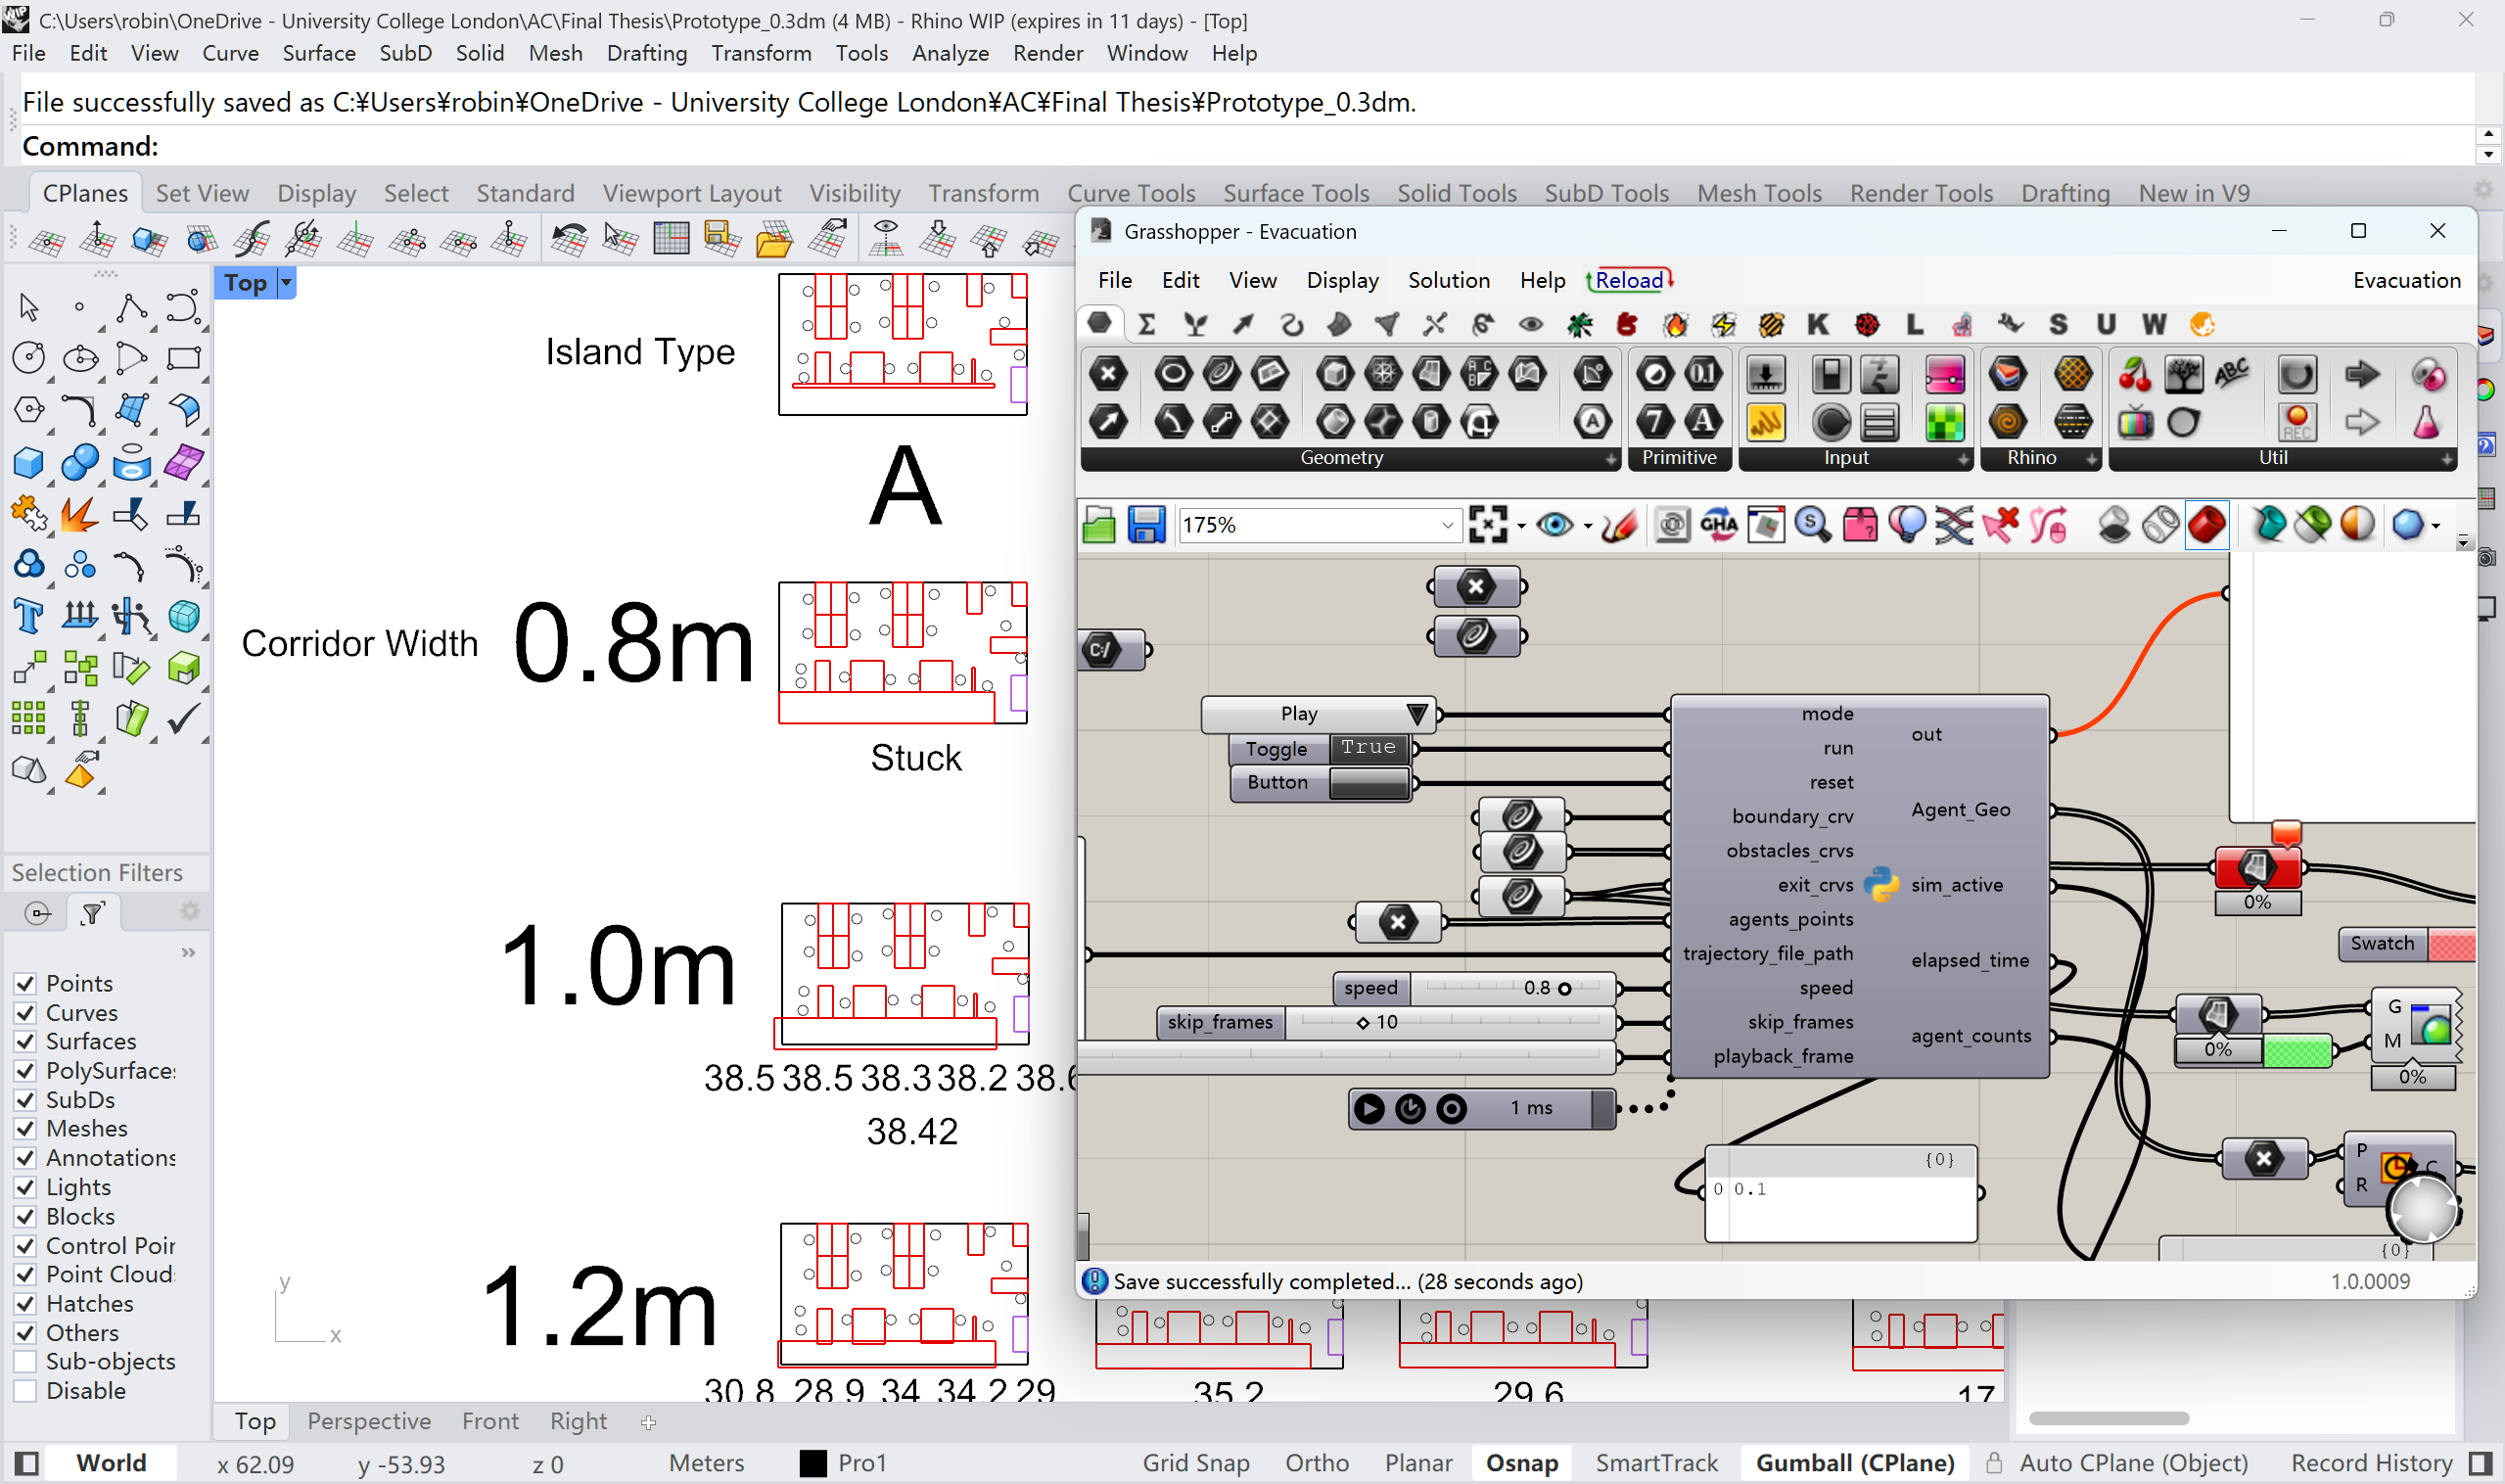
\includegraphics[width=\textwidth]{Rhino&Grasshopper.png}
    \caption{Rhino and Grasshopper}
    \label{fig:rhinoandgrasshopper}
\end{figure}

\section{System Integration}
\subsection{Objectives and Framework}
Standard JuPedSim uses the Shapely package for geometry input and visualization, which limits efficiency when generating multiple experimental prototypes and offers limited parametric control. This study based on Rhino3D's parametric modeling environment,using a Python script \ref{fig:pythonscript} to integrate geometric data and call JuPedSim's API to run the simulation, in order to conveniently generate prototypes and systematically control parameters during each experiment.

\subsection{Input and Output Description }
As the figure \ref{fig:pipeline} shows, Geometric inputs define the physical space through polyline(stored as point list) representations of the office layout, including office space boundaries that establish the walkable area, obstacle geometries that represent furniture or colunms, and exit locations. Additionally, the system requires agent positioning data provided as a point list that specifies the initial locations where pedestrians will be placed before the simulation. 

Each simulation run generates an individual SQLite file that stores all simulation results. The file stores trajectory data including frames, agent id, agent coordinates per frame, and orientation vectors per frame. The file also preserves simulation metadata and geometric data of the walkable area, allowing subsequent analysis and playback.'

\begin{figure}[h]
    \centering
    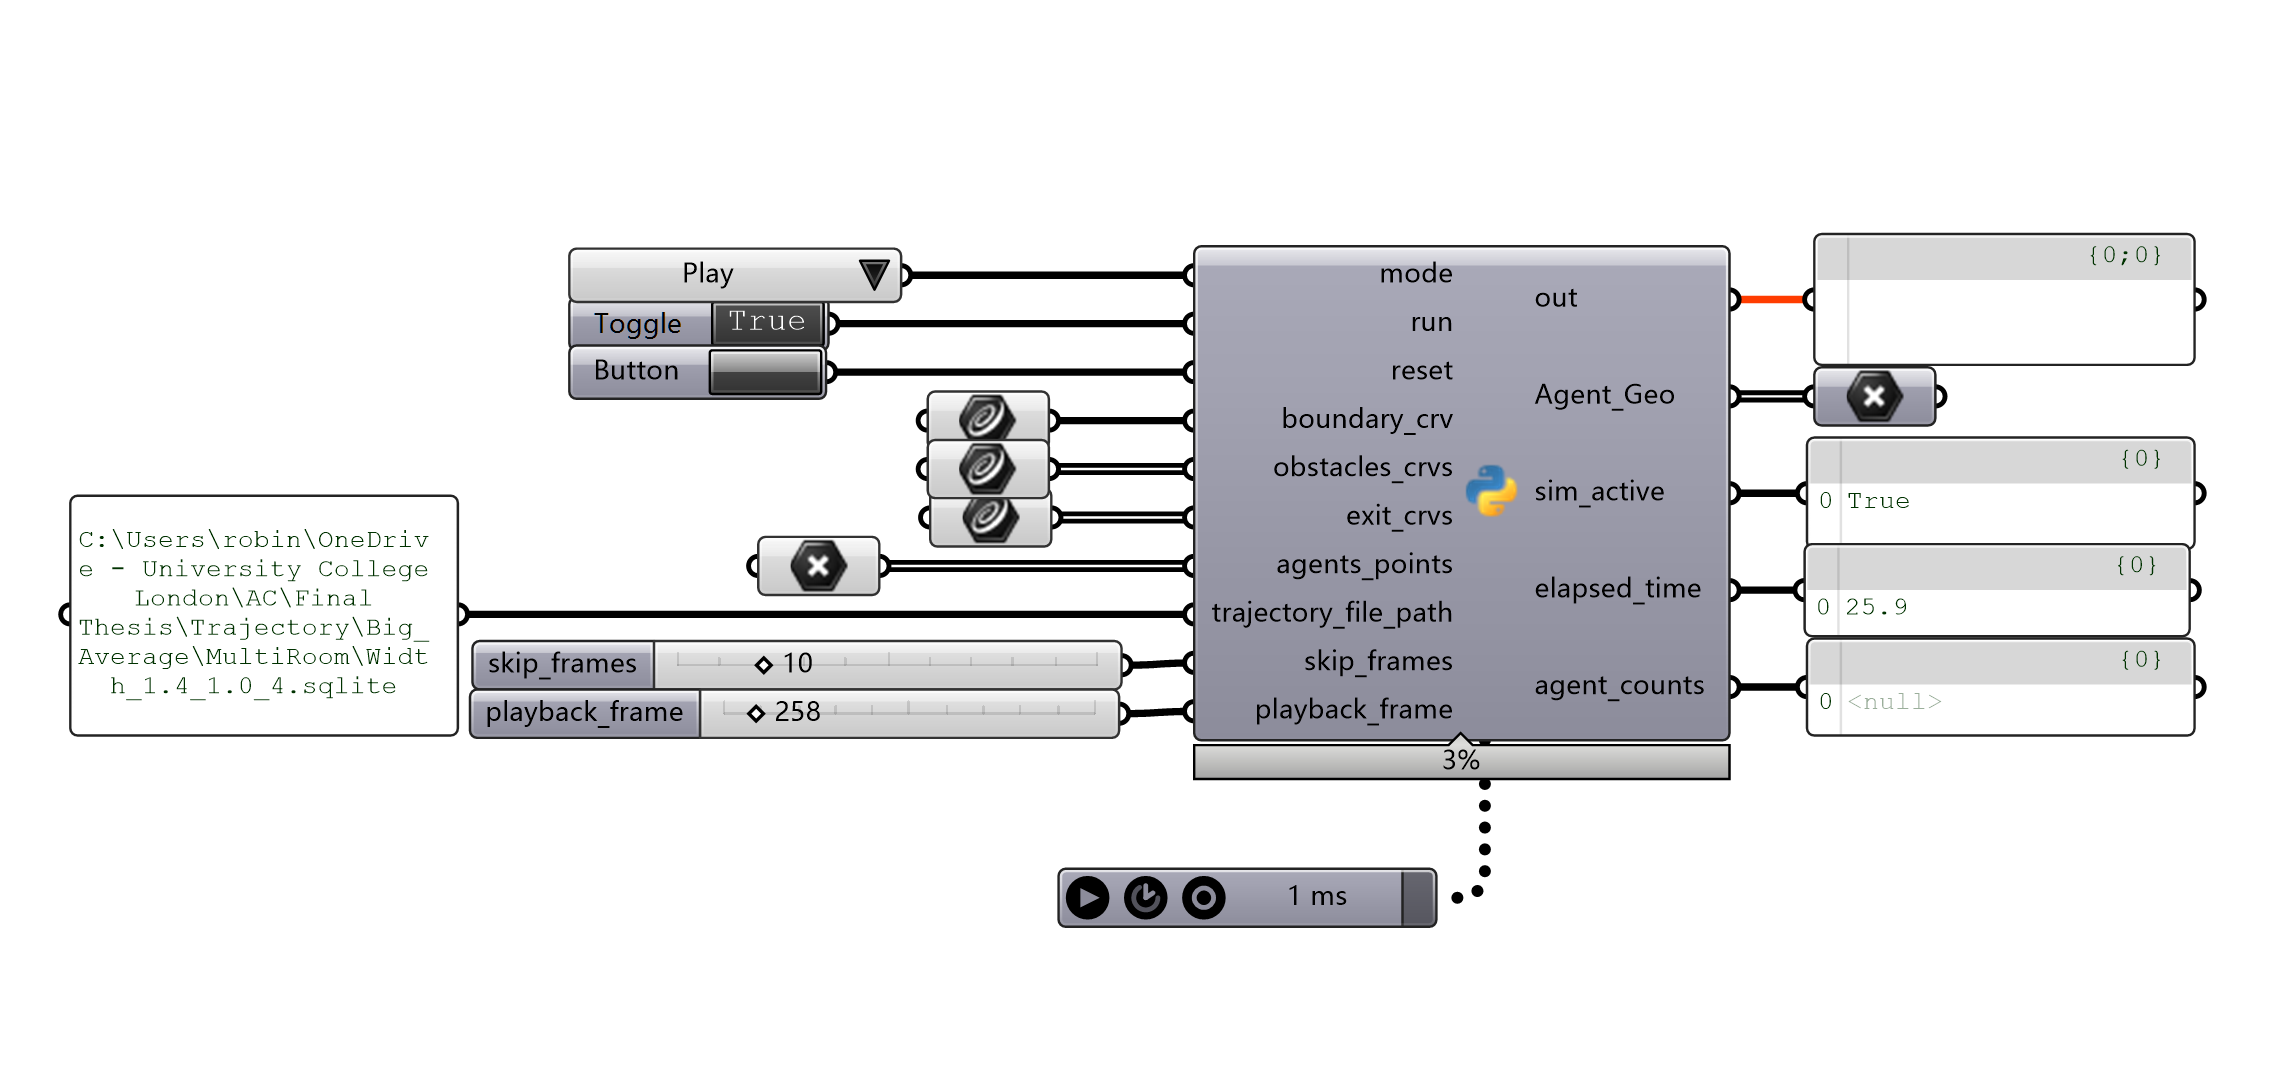
\includegraphics[width=\textwidth]{PythonScript.png}
    \caption{Python Script in Grasshopper for JuPedSim Integration}
    \label{fig:pythonscript}
\end{figure}

\begin{figure}[h]
    \centering
    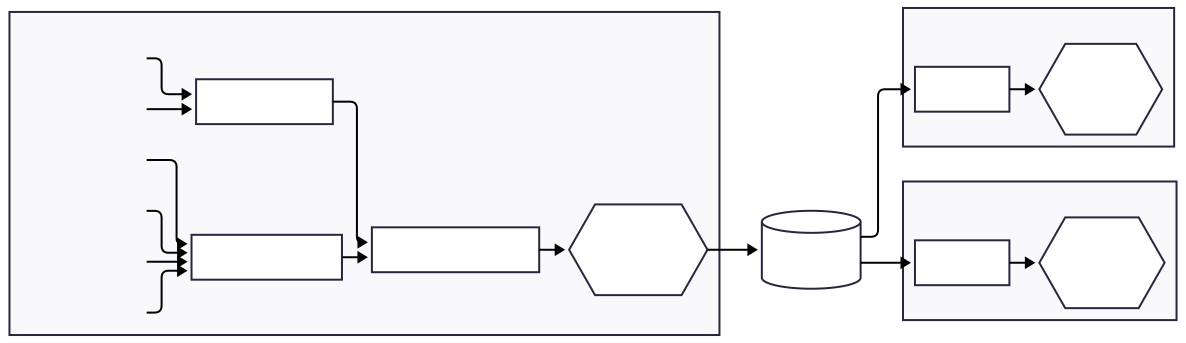
\includegraphics[width=\textwidth]{DataPipeline}
    \caption{Data Pipeline}
    \label{fig:pipeline}
\end{figure}

\section{Experimental design}

\subsection{Prototype Scales}
Small prototype \ref{fig:small} focus on the preliminary effects of layout on evacuation paths and times. To eliminate the influence of multiple corridors, we extended the bottom wall to the leftmost and bottommost sides, keeping only the Main corridor while controlling its width.
\begin{figure}[h]
    \centering
    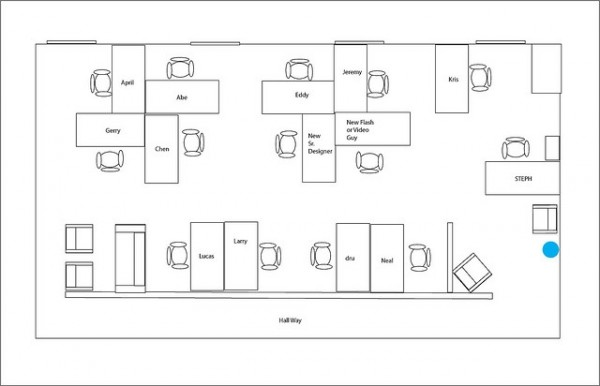
\includegraphics[width=\textwidth]{Small.jpg}
    \caption{Small Prototype Primitive}
    \label{fig:small}
\end{figure}

Big prototype \ref{fig:big} introduces higher-level issues such as bottleneck limitations and coupling effects of room door width and corridor gate width, testing at a scale closer to actual office spaces.
\begin{figure}[h]
    \centering
    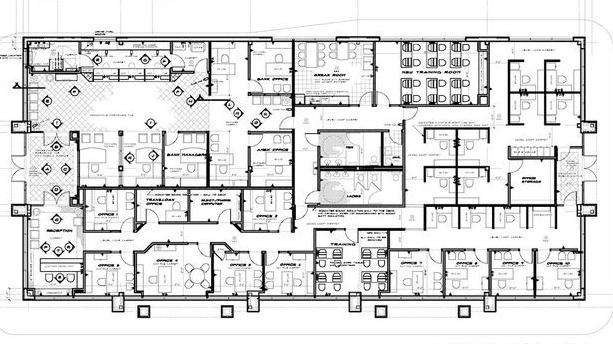
\includegraphics[width=\textwidth]{Big.jpg}
    \caption{Big Prototype Primitive}
    \label{fig:big}
\end{figure}

\subsection{Randomness and Replication}
Each parameter configuration is repeated 5 runs, and each run is stored as an individual SQLite file. For each run, initial agent positions are randomly moved by a method, which can be described by the following pseudo code:
\begin{listing}[H]
    \caption{Random Start Position Function}
    \label{Algo:randompoint}
    \begin{algorithmic}[1]
        \Function {$RandomPoint$}{point, seed}
        \State $random \gets RandomNumberGenerator(seed)$
        \State $randomX \gets random.uniform(-0.1, 0.1)$
        \State $randomY \gets random.uniform(-0.1, 0.1)$
        \State $newPoint \gets (point.X + randomX, point.Y + randomY)$
        \State \Return $newPoint$
        \EndFunction
    \end{algorithmic}
\end{listing}

\subsection{Small Prototype Variables}
Table Layout \ref{fig:abc} includes three variants A, B, and C to represent the internal furniture configuration.
\begin{figure}[h]
    \centering
    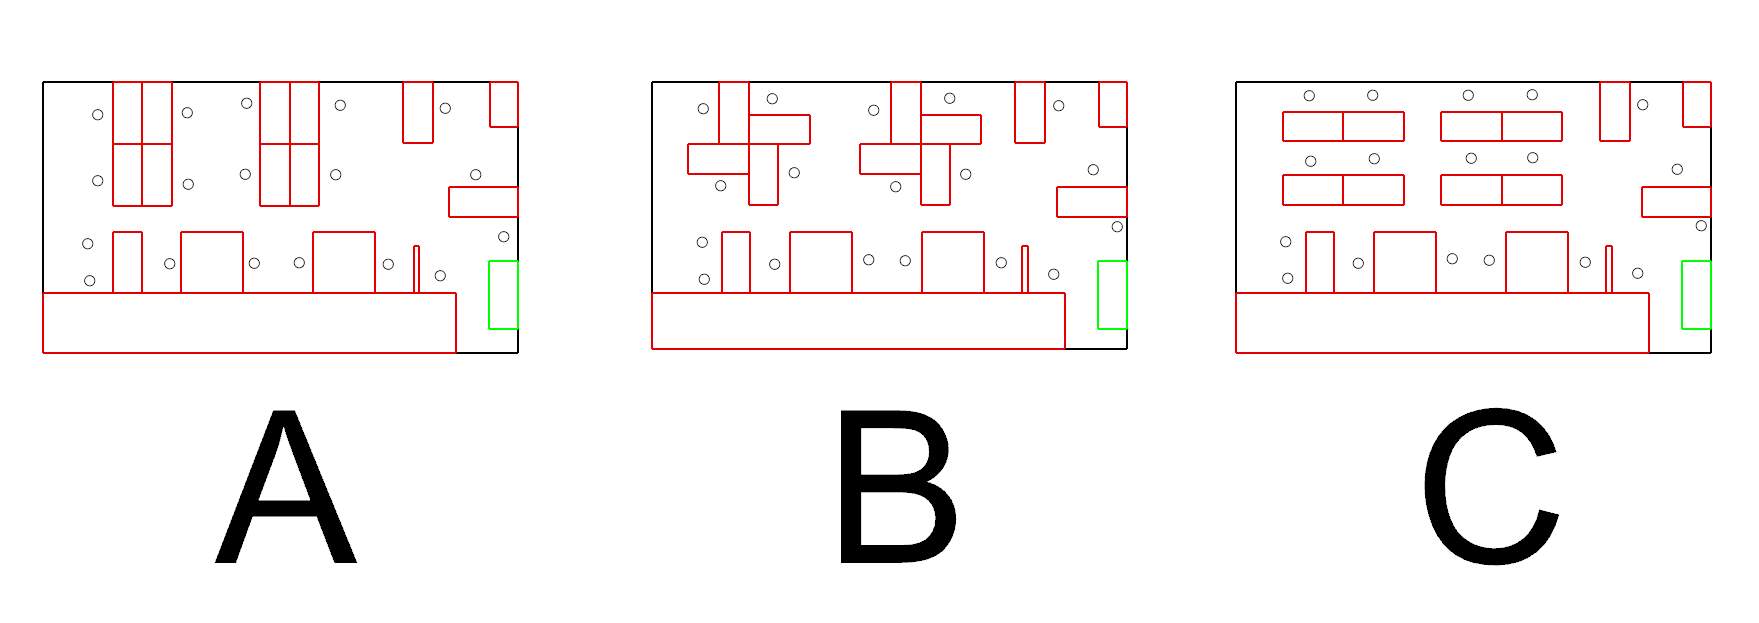
\includegraphics[width=\textwidth]{abc.png}
    \caption{Three Types of Table Layout}
    \label{fig:abc}
\end{figure}

Corridor Width \ref{fig:corridorwidth} ranges from 0.8 m to 2.4 m (step 0.2 m), in order to systematically vary the available passage space, where width is measured as the perpendicular distance from the bottom edge of the upper furniture to the top edge of the lower furniture.  
\begin{figure}[h]
    \centering
    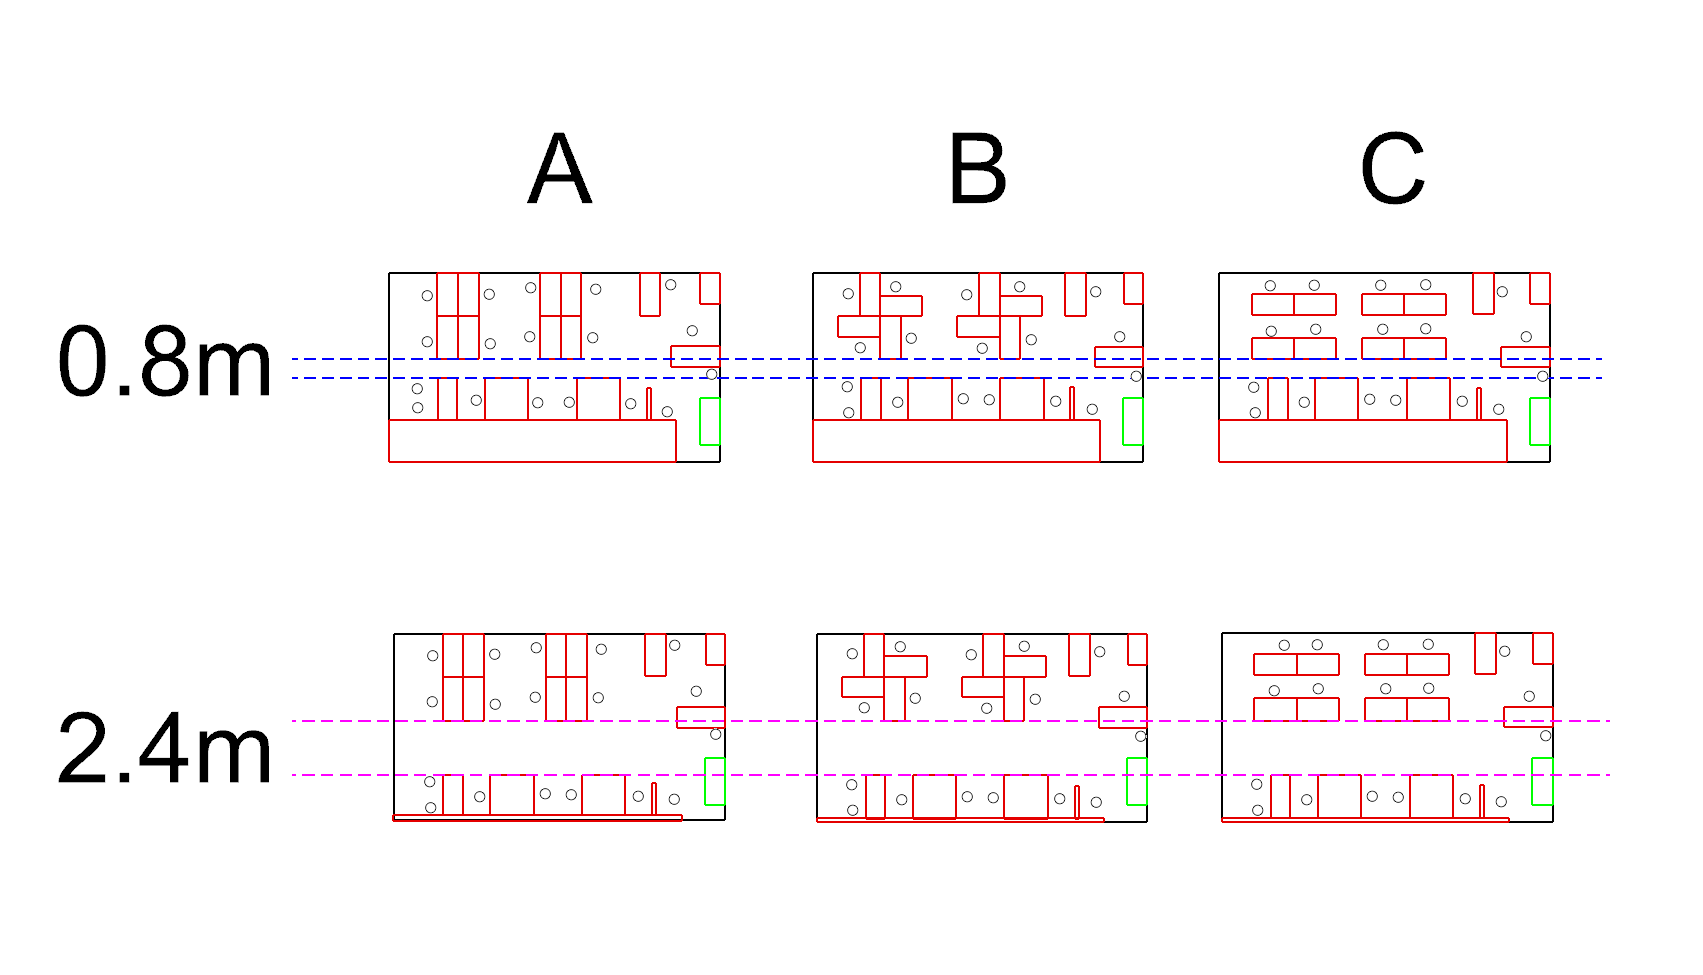
\includegraphics[width=\textwidth]{WidthCompare.png}
    \caption{Corridor Width}
    \label{fig:corridorwidth}
\end{figure}

Besides the single exit configuration, double exit arrangements are served as an add-on experiments metric across all corridor width and table layout variables. This parallel design allows comparison of flow and congestion patterns in different path choices. 
\begin{figure}[h]
    \centering
    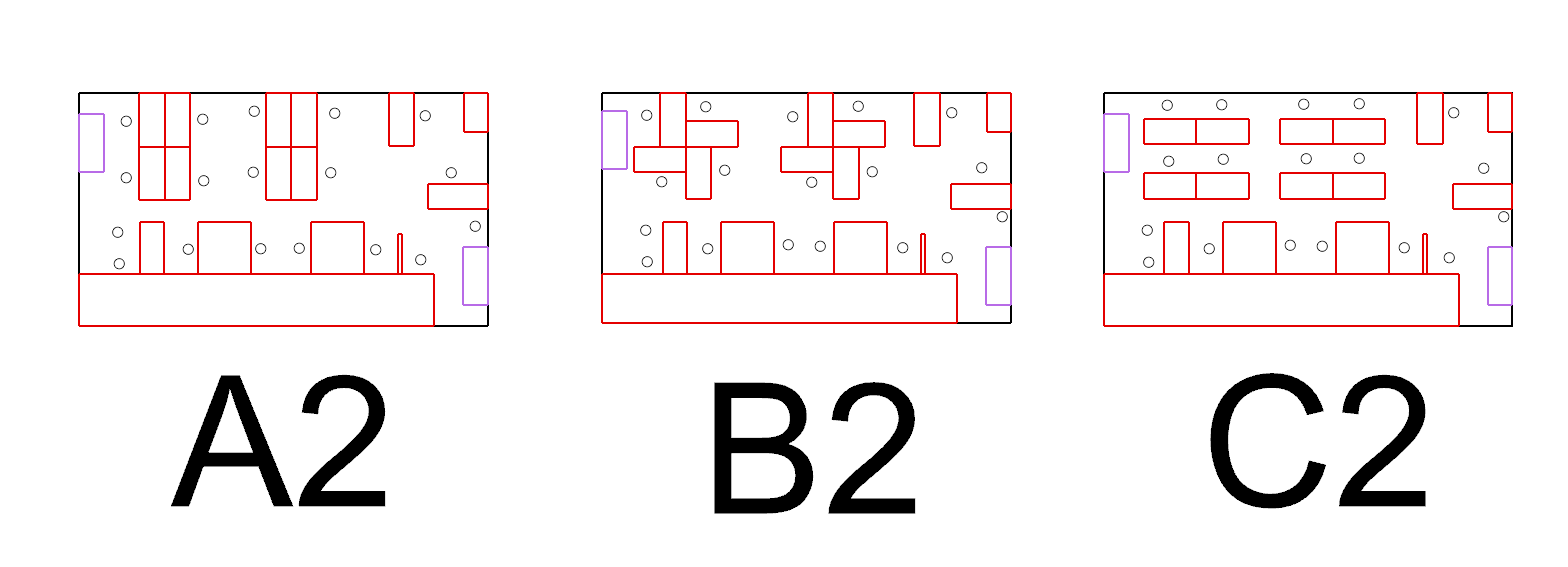
\includegraphics[width=\textwidth]{abc2.png}
    \caption{Exit Configuration}
    \label{fig:ExitConfiguration}
\end{figure}

\subsection{Big Prototype Variables}
The study firstly conducted a primitive simulation on the original big prototype. And then based on the initail trajectories, we designed two main variable groups:

Gate width before the exit(the bottleneck) \ref{fig:4ExitsGate} is varied from 1.0 m to 1.6 m (steps 0.2 m), in order to systematically assess the affects of early queuing, discharging, and lane merging. The range is chosen based on common architectural standards for exit widths \cite{linSimulatingEffectsGate2023}, ensuring that the variations are realistic to typical office environments. 

According to the primitive simulation \ref{fig:bigprimitive}, with red curves in the figure representing agent trajectories from all the five runs, the trajectories show convergence into three main corridor segments: corridor a (upper), corridor b (lower-left), and corridor c (lower-right). To quantify the combined effects of room entrance(blue) and corridor gate(red) on the flow distribution and congestion of these main passages, we conducted a experiment using room door width and corridor gate width as core variables, ranging from 1.0 m to 1.6 m (step 0.2 m). For each combination, we evaluated its impact on queuing, throughput capacity, and the merging and conflict patterns. 

\begin{figure}[h]
    \centering
    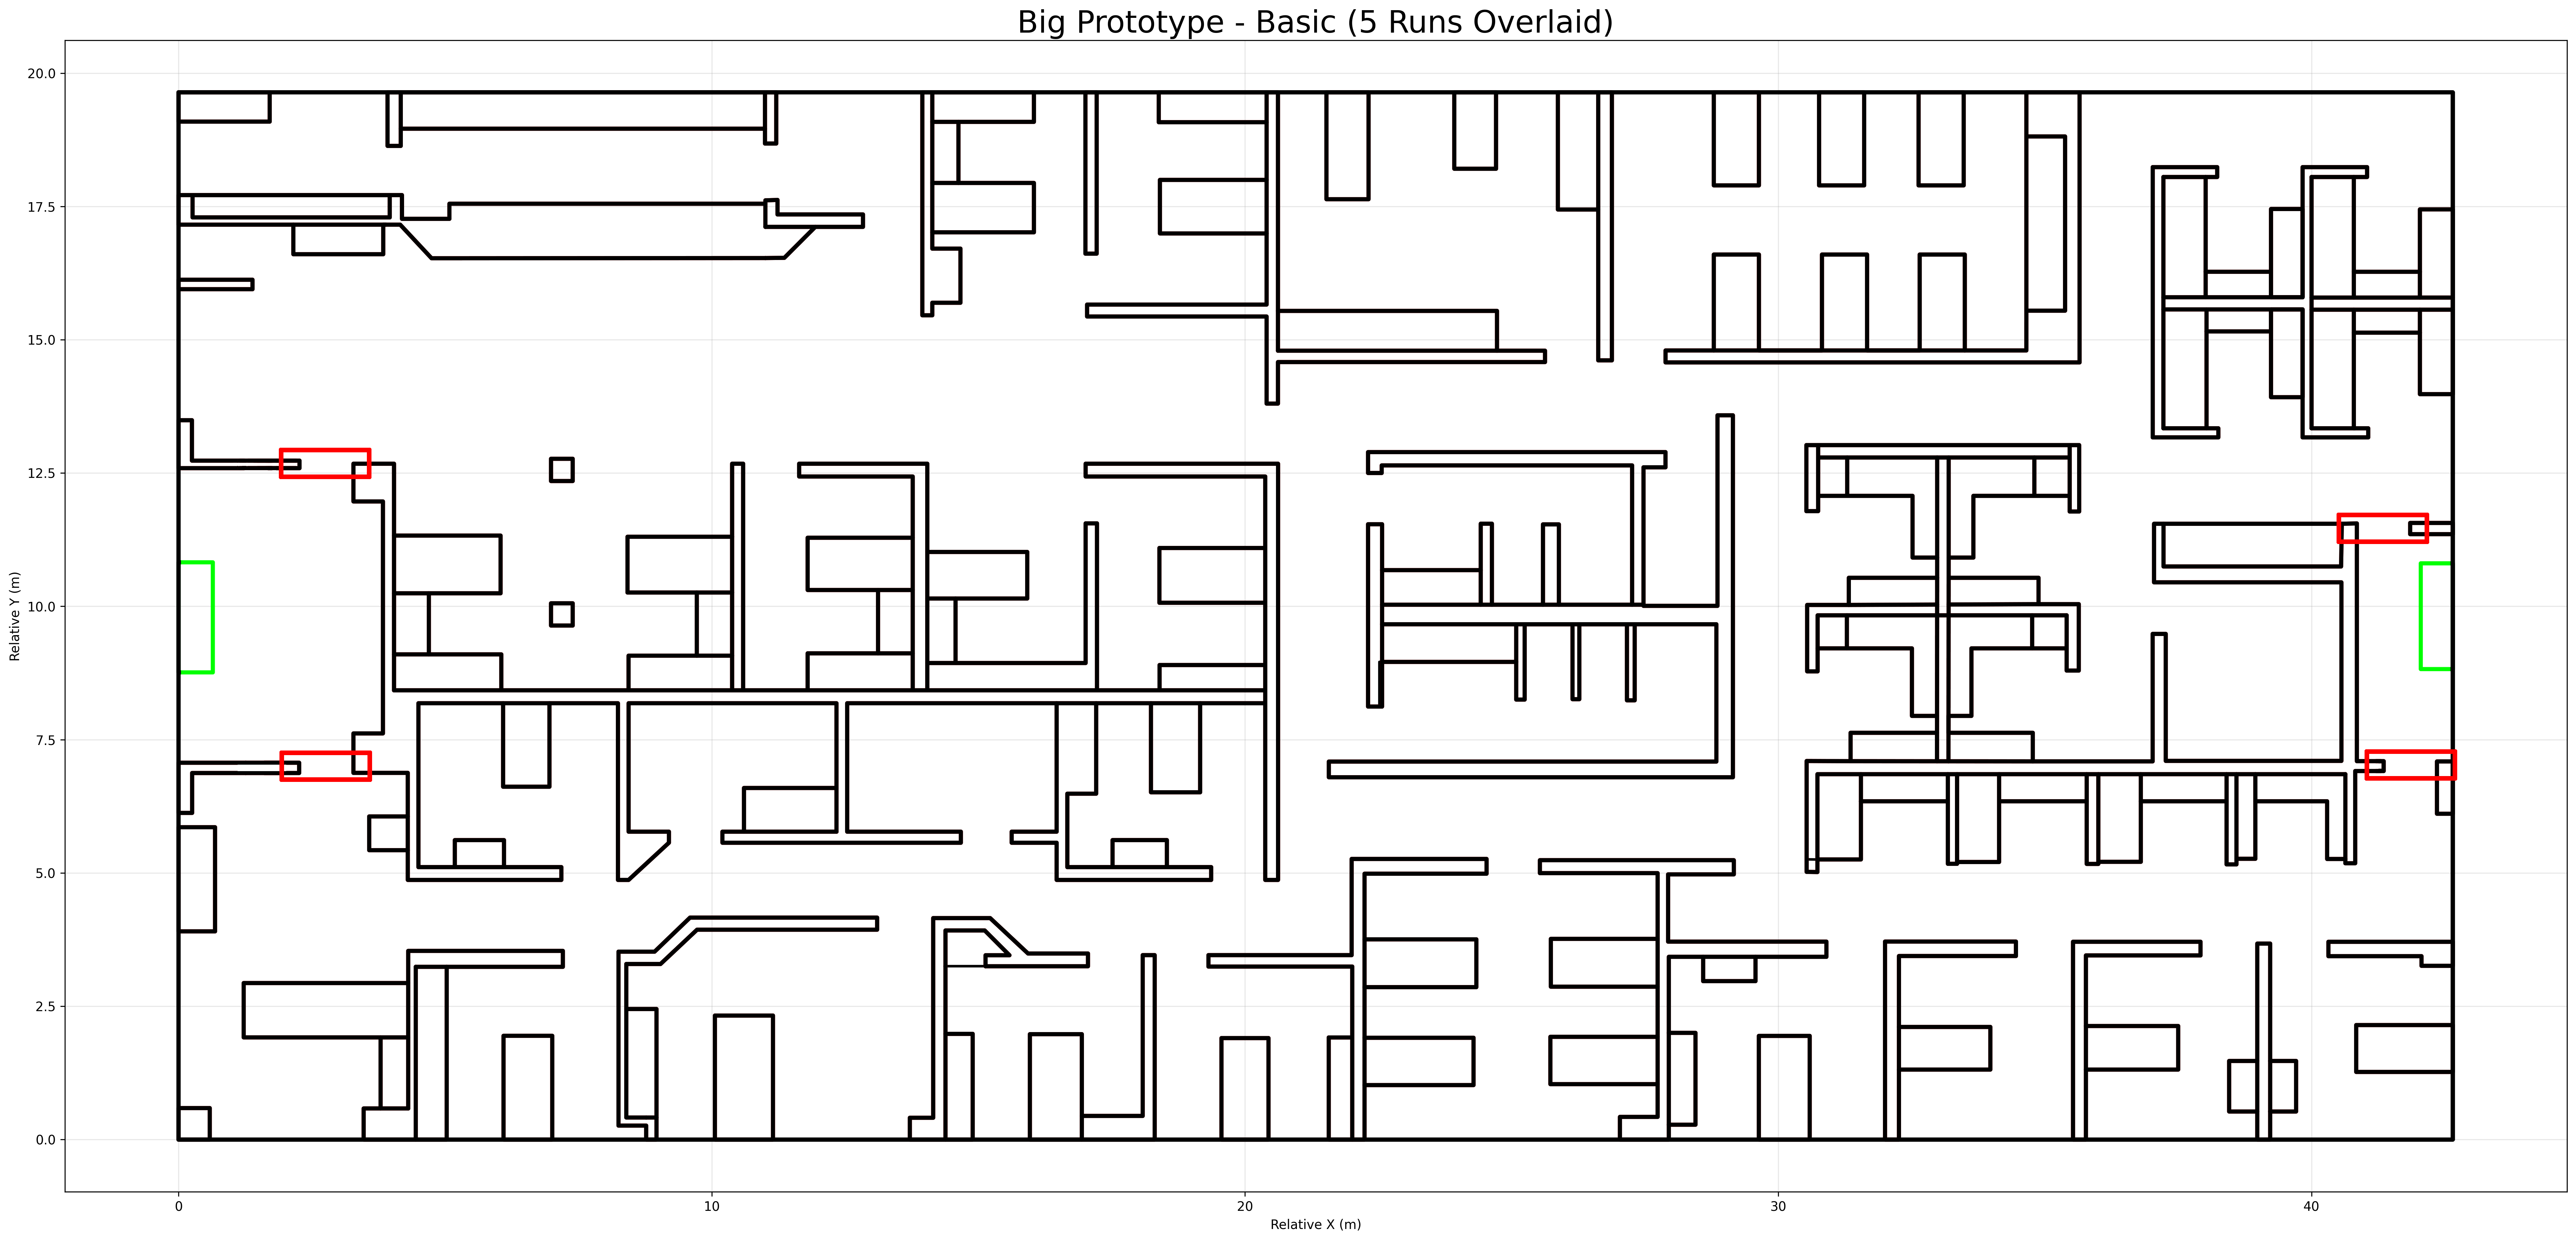
\includegraphics[width=\textwidth]
    {trajectory_overlay_layout_4ExitsGate.png}
    \caption{Change of the gates width before the exits}
    \label{fig:4ExitsGate}
\end{figure}

\begin{figure}[h]
    \centering
    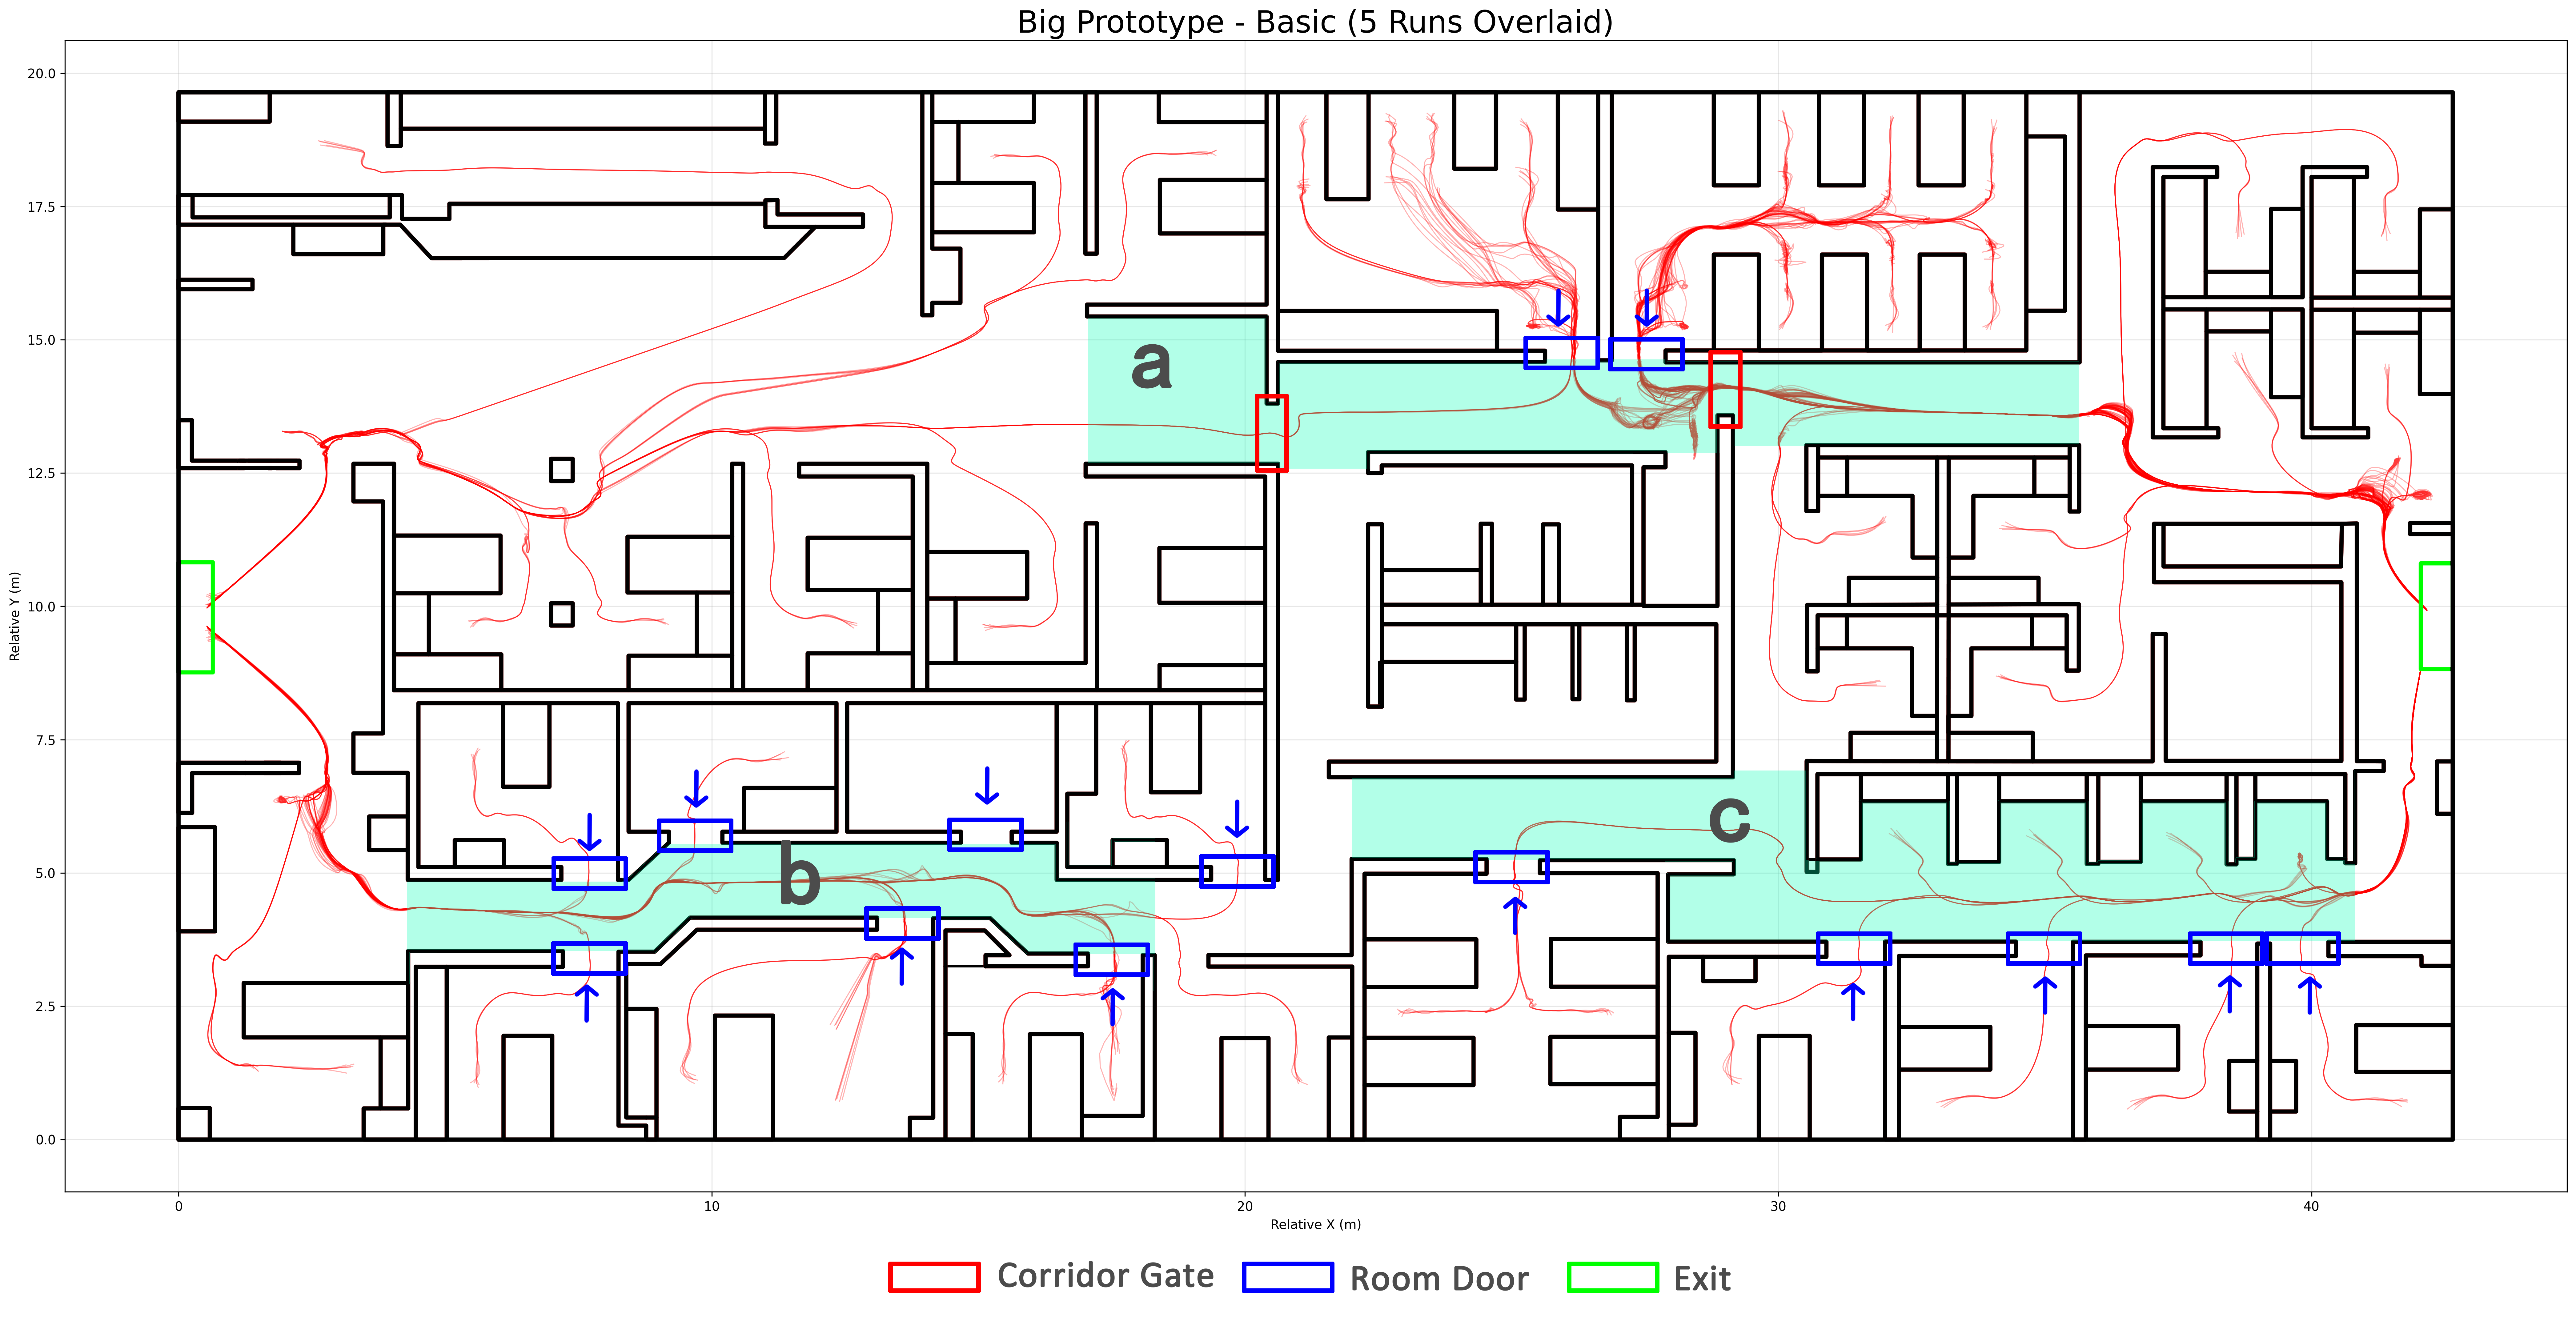
\includegraphics[width=\textwidth]{trajectory_overlay_layout_CorridorAnalysis_Basic.png}
    \caption{Trajectories on the original big prototype and main corridor segments}
    \label{fig:bigprimitive}
\end{figure}

\begin{figure}[h]
    \centering
    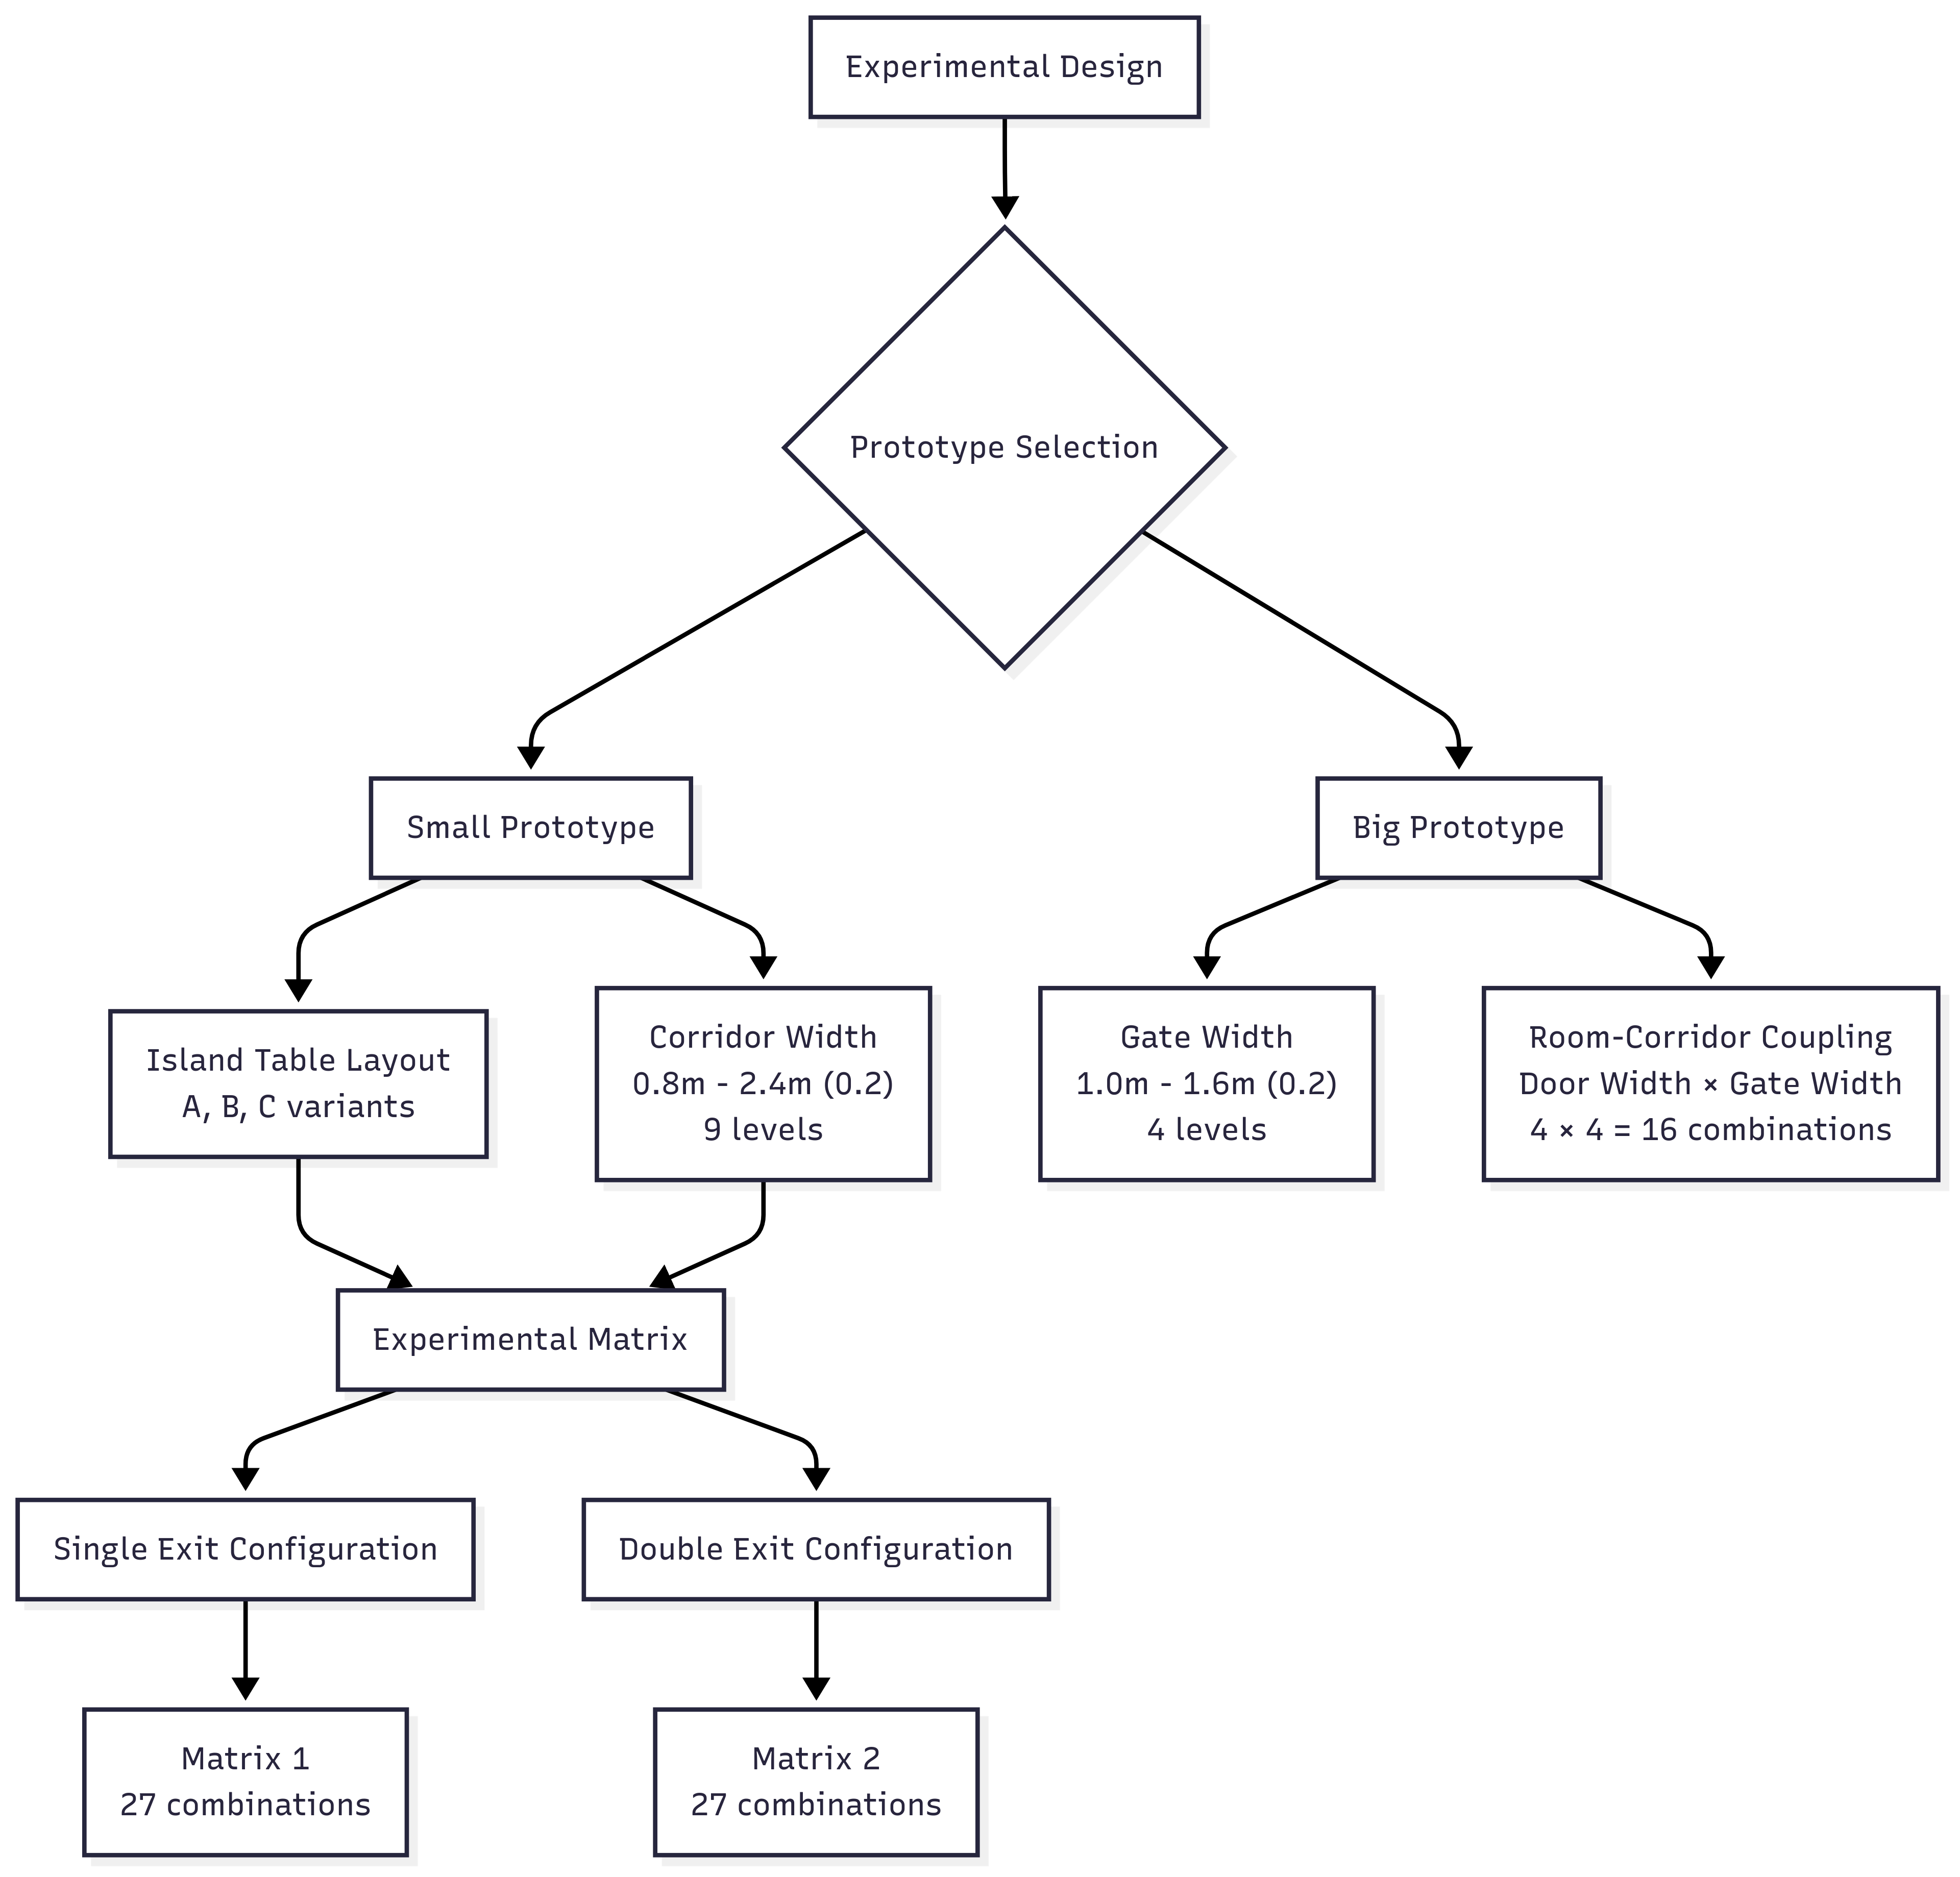
\includegraphics[width=\textwidth]{ExperimentalDesign.png}
    \caption{Experimental Design}
    \label{fig:experimentaldesign}
\end{figure}

\section{Agents and Model Settings}

The built-in Social Force Model of JuPedSim is used as the simulation model, whose defult parameters are set as follows:

\begin{listing}[H]
    \caption{Social Force Model Parameters}
    \label{lis:SFMparameters}
    \begin{minted}[firstnumber=1,breaklines]{Python}
        SocialForceModel(
            body_force: float = 120000, 
            friction: float = 240000)
    \end{minted}
\end{listing}

These include repulsive forces between agents, repulsive forces against obstacles, and response intensity to queuing and group aggregation. The initial settings adopt the official recommended values from JuPedSim.

And agent parameters are adjusted to fit the experiments, which are set as follows:

\begin{listing}[H]
    \caption{Social Force Model Agent Parameters}
    \label{lis:SFMAgentparameters}
    \begin{minted}[firstnumber=1,breaklines]{Python}
        SocialForceModelAgentParameters(
            position: tuple[float, float] = agent_start_postion, 
            orientation: tuple[float, float] = (0.0, 0.0),
            journey_id: int = assigned_journey_id, 
            stage_id: int = closet_exit_id, 
            velocity: tuple[float, float] = (0.0, 0.0), 
            mass: float = 80.0, 
            desired_speed: float = 0.8, 
            reaction_time: float = 0.5, 
            agent_scale: float = 2000, 
            obstacle_scale: float = 1000, 
            force_distance: float = 0.08, 
            radius: float = 0.3)
    \end{minted}
\end{listing}

The total number of agents is set in the Rhino3D scene based on the seat quantity of the two scale prototypes. In our case, the small prototype has 18 agents, and the big prototype has 57 agents. The point list of Grasshopper is mapped to the initial positions of the agents, with the random start position function \ref{Algo:randompoint}.

In scenarios with multiple entrances, agents tend to choose the shortest path. To simulate the real behavior of people choosing the nearest exit, we suppose that each agent would choose the $\text{straight-line distance}$ to the nearest exit as their target, and set the $\text{stage\_id}$ parameter accordingly. Because when we are in a building, we can not accurately calculate the distance to exits, but we can roughly judge which exit is closer.

The defult desired speed of JuPedSim is 0.8m/s, and this study also trys to find a fitable desired speed. Helbing et al. discovered the "faster is slower" effect. When desired speeds exceed 1.5 m/s, it reduces evacuation time by 25\% \cite{helbingSimulatingDynamicalFeatures2000}. We firstly tested the 0.8-1.5 m/s speed range according to Helbing's theoretical predictions, and agents at desired speed of 0.8 m/s showing more orderly behavior. Because this speed falls within normal walking conditions, avoiding the disorderly pushing phenomena triggered by high desired speeds. Therefore, we keep the desired speed as defult.

The obstacle force scale is set to 1000, in order to balance the resistance to obstacles in complex scenarios, preventing excessive suppression of agent movement. Boundary conditions follow the wall and exit definitions in the geometric input of the scene.

\section{Data collection and Analysis}

\subsection{Data Reading and Processing}
The study uses JupyterLab and Python to read SQLite files, organizing the data into an analyzable structure, and visualizing the data by tables, line charts, speed-trajectory diagrams and heat maps.

\subsection{Indicators}

The main indicators for checking evacuation performance include the Total Evacuation Time (hereinafter referred to as TET),Path fistribution and Congestion hotspot distribution. Total Evacuation Time is the most important measure for comparing how evacuations perform in different settings, usually shown through time tables and line charts. Path distribution show how people move during evacuation through movement patterns in speed-trajectory diagrams, giving clear information about how evacuation flows develop and spread during the evacuation process. Also, Congestion Hotspot Distribution analysis focuses on finding where and how much slow-moving crowds and crowded areas appear in speed-movement diagrams, which also shows crowded spots and tracks how they move during evacuation.

Besides, the rebustness of the evacuation performance is also considered, which is reflected in the fluctuation range of TET under multiple runs of the same parameter configuration. A smaller fluctuation range indicates a more stable evacuation performance. 

\subsection{Results Presentation and Visualization}
This study uses Total Evacuation Time (TET) as the primary evaluation metric. For each parameter level (such as door width, corridor width, and exit configuration), we calculate the mean TET and fluctuation range from multiple independent simulations, and conduct direct comparisons and ranking based on these results. To identify potential threshold effects, we observe slope changes in evacuation time line graphs, record parameter intervals where significant inflection points or plateau segments occur, and select representative parameter points to compare with speed-trajectory diagrams to explain the mechanistic differences in congestion patterns as parameters vary. 